This layer is responsible for providing necessary power for the instrument. It mainly consists of 12V 2A DC batteries or regular 120V AC current can be used for this layer.
\subsection{Layer Hardware}
There is no specific hardware required for this layer except of combination 12V batteries and the outlet cord for AC supply . This layer is merely acting as an power source for the raspberry pi, lasers' circuit, teensy micro-controller and mister. 


\subsection{Battery/AC outlet}
It consists of 12V 2A DC batteries' combination or AC outlet along with hookup and jumper wires for connection to the pi and the breadboard.

\begin{figure}[h!]
	\centering
 	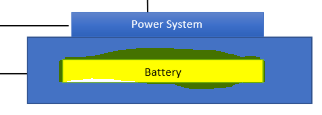
\includegraphics[width=0.60\textwidth]{images/Capture.png}
 \caption{Power layer subsystem diagram}
\end{figure}



